\chapter[Spatiotemporal separation of PER and CRY posttranslational regulation]{Spatiotemporal separation of PER and CRY posttranslational regulation\footnote{Portions of this chapter are published in P. C. St. John, T. Hirota, S. A. Kay, and F. J. Doyle III, ``Spatiotemporal separation of PER and CRY posttranslational regulation in the mammalian circadian clock.,'' {\itshape Proc. Natl. Acad. Sci. U. S. A.}, vol. 111, pp. 2040–5, Feb. 2014.}}\label{chap:longdaysin}

In the previous chapter, computationally efficient techniques for preforming a bootstrap analysis on circadian models was described. 
In this chapter, we apply this technique to clarify the roles of two posttranslational regulators in the core circadian feedback loop. 
Since direct experimental evidence of the systems-level effect of these regulators is difficult if not impossible to obtain, we must rely on computational modeling to provide insight into the dynamic consequences of modulating posttranslational activity. 
For this reason, bootstrap methods are invaluable in generating confident {\itshape in silico} results. 

\section{Background}

Since circadian and metabolic regulators are tightly integrated, circadian disruptions often manifest in metabolic disease \cite{Bass2012}. 
Recent efforts have therefore sought to gain a mechanistic understanding of these pathways, such that the metabolic burdens imposed by a 24-hour society might be mitigated. 
Posttranslational regulators, which play key roles in connecting circadian and metabolic processes, serve as likely targets for future therapeutics -- demonstrated by the wealth of available circadian-active small molecules \cite{Chen2013}.

\subsection{Nuclear entry of PER-CRY complex}
% Oscillations in circadian gene transcription are generated through a time-delayed transcription-translation negative-feedback loop. 
% In mammals, transcription factors CLOCK and BMAL1 promote transcription of E box-containing genes {\it Period} ({\it Per}) and {\it Cryptochrome} ({\it Cry}) (\fref{fig:4-1a}). 
% PER and CRY protein products form heterodimers to accumulate in the nucleus, in which PER is stoichiometrically limiting \cite{Lee2001}, and subsequently close the negative feedback loop by inhibiting CLOCK-BMAL1-promoted gene expression. 
% While steady-state endpoint assays have shown the possibility of nuclear entry of CRY without PER \cite{Ye2011, Kume1999, Yagita2002}, experiments from {\it Per1}\textsuperscript{-/-} {\it Per2}\textsuperscript{-/-} mice demonstrated that PER proteins are required for the timely nuclear accumulation of CRY \cite{Lee2001}. 
% Clearance of nuclear repressors reactivates CLOCK-BMAL1, allowing the cycle to begin anew \cite{Takahashi2008}. 

Experimental evidence on PER/CRY nuclear entry is seemingly contradictory. 
For nuclear localization of the PER and CRY proteins, experiments from {\it Per1}\textsuperscript{-/-} {\it Per2}\textsuperscript{-/-} mice demonstrate that PER proteins are required for timely nuclear accumulation of CRY \cite{Lee2001}. 
While other studies have shown the possibility of nuclear entry of CRY without PER, these results are typically based on steady-state endpoint assays which do not consider the speed of CRY nuclear entry \cite{Ye2011, Kume1999, Yagita2002}. 
We therefore consider the formation of the PER-CRY heterodimer as a key step in nuclear entry, which is supported by the fact that to the best of our knowledge all circadian models that consider both PER and CRY employ this kinetic assumption \cite{Hirota2012, Relogio2011, Leloup2003, Forger2003, Mirsky2009}.

\subsection{Importance of posttranslational regulators}
The stabilities of PER and CRY are tightly regulated: PER proteins are phosphorylated by the casein kinase we family of proteins (CKI$\delta/\epsilon$), prompting $\beta$-TrCP-mediated degradation \cite{Reischl2007} and nuclear import \cite{Takano2004}. 
The degradation of CRY proteins is separately regulated by the SCF\textsuperscript{FBXL3} ubiquitin ligase complex \cite{Busino2007, Godinho2007, Siepka2007}. 
The activities of both CKI-PER and FBXL3-CRY may be further coupled to the cell's metabolic state through AMPK signalling \cite{Lee2013}. 
These posttranslational regulatory mechanisms have a strong effect on period length: the gain-of-function mutant CKI$\epsilon^\mathrm{tau}$ leading to hyperphosphorylation of PER \cite{Gallego2006} and small molecule CKI inhibitors, such as longdaysin \cite{Hirota2010}, demonstrated that increasing or decreasing CKI-dependent PER phosphorylation shortens or lengthens the period, respectively. 
In contrast, genetic mutations of FBXL3 \cite{Godinho2007, Siepka2007} and KL001, a small molecule inhibitor of FBXL3-dependent CRY degradation \cite{Hirota2012}, showed that increased CRY stability leads to longer periods. 
Since the scale and complexity of the circadian network complicates an intuitive understanding of these relationships, mathematical models have played important roles in understanding how these manipulations affect circadian period \cite{Gallego2006, Hirota2012, Reischl2007}.

\subsection{Functional differences between PER and CRY}
Given that both CKI and FBXL3 pathways regulate the stability of linked negative factors, it was thought that simultaneous perturbations to both pathways might lead to non-additive effects: i.e., the slowest link would determine the period. 
 However, both small molecule \cite{Hirota2012} and genetic experiments \cite{Maywood2011} have demonstrated the independent period effects of these two posttranslational regulations. 
A recent clarification of the canonical clock feedback circuit has shown that dissociated CRY is the dominant repressor of CLOCK-BMAL1 mediated E box transcription \cite{Ye2011}. 
This distinction helps differentiate between the roles of the otherwise similar PER and CRY proteins, in which the main role of PER in transcriptional repression is likely regulating the timing of nuclear accumulation of CRY. 
Therefore, while previous mathematical models in which PER acts as a direct repressor have proposed mechanisms for CKI-dependent period lengthening \cite{Gallego2006, Vanselow2006}, they are likely not suitable for distinguishing between CKI-PER and FBXL3-CRY mediated period change.

In this chapter, we used human cells harboring clock gene reporters together with mathematical modeling to gain insight into the relationship between PER and CRY posttranslational regulation. 
Consequently, we provide a new mechanism by which CKI-dependent PER phosphorylation controls the circadian period separately from the FBXL3-CRY pathway. 
The resulting detailed understanding of PER and CRY regulation in the core feedback loop provides a framework on which to interpret metabolic and pharmacological control of circadian rhythms.

\section{Methods}
\subsection{Analysis of luminescence profiles}
Raw luminescence data was first separated into a moving baseline and oscillatory component using a Hodrick-Prescott filter with a smoothing parameter of 1600. 
Example trajectory decompositions are shown in \fref{fig:4s1}. 
Amplitudes (as shown in \fref{fig:4-1b}) were determined by taking the standard deviation in the baseline-subtracted data. 
Periods were obtained by nonlinear curve fitting, in which a four parameter (initial amplitude, decay, period and phase) damped cosine curve was fit to the baseline-subtracted data. 
Periods were not shown if the relative amplitude (found by standard deviation) fell below 25\%, since noise dominated the periodic trajectory. 

\begin{figure}[p]
  \centering
  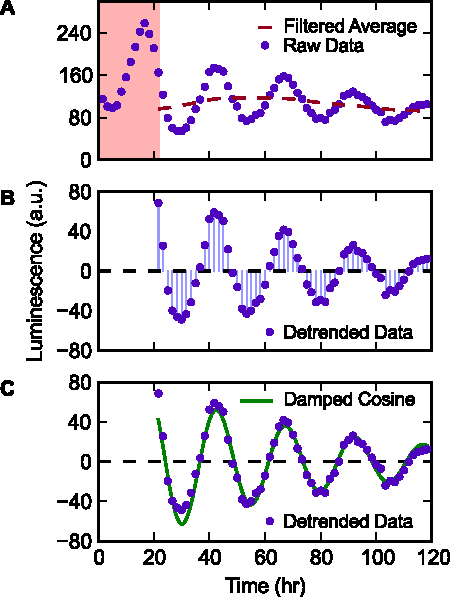
\includegraphics[width=0.6\textwidth]{chap4/figures/figS1.pdf}
  \titlecaption{Analysis of circadian reporter luminescence data}{ ({\bfseries A}) Raw luminescence data is first cropped by removing the initial transient region (first 12 points). The moving baseline is estimated using a Hodrick-Prescott filter with smoothing parameter 1600 (red dashed line). ({\bfseries B}) Data is detrended by subtracting the moving baseline from the raw data. The detrended data is used to calculate the relative amplitude of the oscillations via standard deviation. ({\bfseries C}) Periods are estimated by fitting a damped cosine curve (green solid line) to the detrended data. Figure reprinted from \cite{St.John2014}.}
  \label{fig:4s1}
\end{figure}

\subsection{Cost function}
Models were fit to a cost function of experimental results. 
{\it Per}, {\it Cry}, {\it Clock}, and {\it Bmal1} protein and mRNA levels were taken from \cite{Lee2001}, along with profiles of CRY nuclear localization. 
For the model from \cite{Relogio2011}, additional activity profiles on {\it Rev-Erb} and {\it Ror} were obtained from CircaDB (\url{http://bioinf.itmat.upenn.edu/circa/}). 
To score a model trajectory, mRNA state variables were scaled independently to minimize the squared error between model and experiment, since model parameters could be adjusted to give mRNA profiles arbitrary amplitudes. 
For protein species, where stoichiometric interactions are important, a single scaling parameter was used for all species. 
Nuclear repressor species, in which only relative measurements were available, were scaled independently. 
Full model equations for the model from Hirota {\itshape et al.}, 2012 are shown in \fref{mod:hirota}, the model from Rel\'{o}gio {\itshape et al.} 2011 in \fref{mod:relogioeqs}, and the model from Leloup \& Goldbeter, 2003 in \fref{mod:leloupeqs}.

\begin{model}[p]
  \centering
  \titlecaption{Model from Rel\'{o}gio {\itshape et al.} 2011 \cite{Relogio2011}}{}
  \label{mod:relogioeqs}
  \fontsize{9}{11}

  \begin{align*}
    \frac{d\,\mathit{CLKBM1}}{dt} &= \mathit{BM1n} \cdot \mathit{kfCLKBM1} - \mathit{CLKBM1} \cdot \mathit{dCLKBM1} - \mathit{CLKBM1} \cdot \mathit{kdCLKBM1}\\
    \frac{d\,\mathit{reverb}}{dt} &= \frac{\mathit{V3max} \left(\mathit{g} \cdot
    {\frac{\mathit{CLKBM1}}{\mathit{kt3}}}^{\mathit{v}} +
  1\right)}{{\frac{\mathit{CLKBM1}}{\mathit{kt3}}}^{\mathit{v}}
  {\left(\frac{\mathit{PnCn} + \mathit{PnpCn}}{\mathit{ki3}}\right)}^{\mathit{w}} +
  {\frac{\mathit{CLKBM1}}{\mathit{kt3}}}^{\mathit{v}} + 1} - \mathit{dreverb}
  \cdot \mathit{reverb}\\
  \frac{d\,\mathit{ror}}{dt} &= \frac{\mathit{V4max} \left(\mathit{h} \cdot {\frac{\mathit{CLKBM1}}{\mathit{kt4}}}^{\mathit{p}} + 1\right)}{{\frac{\mathit{CLKBM1}}{\mathit{kt4}}}^{\mathit{p}} \cdot {(\frac{\mathit{PnCn} + \mathit{PnpCn}}{\mathit{ki4}})}^{\mathit{q}} + {\frac{\mathit{CLKBM1}}{\mathit{kt4}}}^{\mathit{p}} + 1} - \mathit{dror} \cdot \mathit{ror}\\
  \frac{d\,\mathit{REVERBc}}{dt} &= - \mathit{REVERBc} \cdot \mathit{dREVERBc} - \mathit{REVERBc} \cdot \mathit{kiREVERBc} + \mathit{kp3} \cdot \mathit{reverb}\\
  \frac{d\,\mathit{RORc}}{dt} &= - \mathit{RORc} \cdot \mathit{dRORc} - \mathit{RORc} \cdot \mathit{kiRORc} + \mathit{kp4} \cdot \mathit{ror}\\
  \frac{d\,\mathit{REVERBn}}{dt} &= \mathit{REVERBc} \cdot \mathit{kiREVERBc} - \mathit{REVERBn} \cdot \mathit{dREVERBn}\\
  \frac{d\,\mathit{RORn}}{dt} &= \mathit{RORc} \cdot \mathit{kiRORc} - \mathit{RORn} \cdot \mathit{dRORn}\\
  \frac{d\,\mathit{bm1}}{dt} &= \frac{\mathit{V5max} \left(\mathit{i} \cdot {\frac{\mathit{RORn}}{\mathit{kt5}}}^{\mathit{n}} + 1\right)}{{\frac{\mathit{REVERBn}}{\mathit{ki5}}}^{\mathit{m}} + {\frac{\mathit{RORn}}{\mathit{kt5}}}^{\mathit{n}} + 1} - \mathit{bm1} \cdot \mathit{dbm1}\\
  \frac{d\,\mathit{BM1c}}{dt} &= - \mathit{BM1c} \cdot \mathit{dBM1c} - \mathit{BM1c} \cdot \mathit{kiBM1c} + \mathit{bm1} \cdot \mathit{kp5}\\
  \frac{d\,\mathit{BM1n}}{dt} &= \mathit{BM1c} \cdot \mathit{kiBM1c} - \mathit{BM1n} \cdot \mathit{dBM1n} - \mathit{BM1n} \cdot \mathit{kfCLKBM1} + \mathit{CLKBM1} \cdot \mathit{kdCLKBM1}\\
  \frac{d\,\mathit{per}}{dt} &= \frac{\mathit{V1max} \left(\mathit{a} \cdot {\frac{\mathit{CLKBM1}}{\mathit{kt1}}}^{\mathit{b}} + 1\right)}{{\frac{\mathit{CLKBM1}}{\mathit{kt1}}}^{\mathit{b}} \cdot {(\frac{\mathit{PnCn} + \mathit{PnpCn}}{\mathit{ki1}})}^{\mathit{c}} + {\frac{\mathit{CLKBM1}}{\mathit{kt1}}}^{\mathit{b}} + 1} - \mathit{dper} \cdot \mathit{per}\\
  \frac{d\,\mathit{cry}}{dt} &= \frac{\mathit{V2max}
  \left(\frac{\mathit{CLKBM1}^{3} \cdot \mathit{d}}{\mathit{kt2}^{3}} +
1\right)}{\left({\frac{\mathit{REVERBn}}{\mathit{ki21}}}^{\mathit{f1}} +
1\right) \left(\frac{\mathit{CLKBM1}^{3}}{\mathit{kt2}^{3}} +
{\frac{\mathit{CLKBM1}}{\mathit{kt2}}}^{\mathit{e}}
{\left(\frac{\mathit{PnCn} +
\mathit{PnpCn}}{\mathit{ki2}}\right)}^{\mathit{f}} + 1\right)} - \mathit{cry}
\cdot \mathit{dcry}\\
\frac{d\,\mathit{Cc}}{dt} &= - \mathit{Cc} \cdot \mathit{Pc} \cdot \mathit{kfPcCc} - \mathit{Cc} \cdot \mathit{Pcp} \cdot \mathit{kfPcpCc} - \mathit{Cc} \cdot \mathit{dCc} + \mathit{PcCc} \cdot \mathit{kdPcCc} + \mathit{PcpCc} \cdot \mathit{kdPcpCc} + \mathit{cry} \cdot \mathit{kp2}\\
\frac{d\,\mathit{Pc}}{dt} &= - \mathit{Cc} \cdot \mathit{Pc} \cdot \mathit{kfPcCc} - \mathit{Pc} \cdot \mathit{dPc} - \mathit{Pc} \cdot \mathit{kphPc} + \mathit{PcCc} \cdot \mathit{kdPcCc} + \mathit{Pcp} \cdot \mathit{kdphPcp} + \mathit{kp1} \cdot \mathit{per}\\
\frac{d\,\mathit{Pcp}}{dt} &= - \mathit{Cc} \cdot \mathit{Pcp} \cdot \mathit{kfPcpCc} + \mathit{Pc} \cdot \mathit{kphPc} - \mathit{Pcp} \cdot \mathit{dPcp} - \mathit{Pcp} \cdot \mathit{kdphPcp} + \mathit{PcpCc} \cdot \mathit{kdPcpCc}\\
\frac{d\,\mathit{PcpCc}}{dt} &= \mathit{Cc} \cdot \mathit{Pcp} \cdot \mathit{kfPcpCc} - \mathit{PcpCc} \cdot \mathit{dPcpCc} - \mathit{PcpCc} \cdot \mathit{kdPcpCc} - \mathit{PcpCc} \cdot \mathit{kiPcpCc} + \mathit{PnpCn} \cdot \mathit{kePnpCn}\\
\frac{d\,\mathit{PcCc}}{dt} &= \mathit{Cc} \cdot \mathit{Pc} \cdot \mathit{kfPcCc} - \mathit{PcCc} \cdot \mathit{dPcCc} - \mathit{PcCc} \cdot \mathit{kdPcCc} - \mathit{PcCc} \cdot \mathit{kiPcCc} + \mathit{PnCn} \cdot \mathit{kePnCn}\\
\frac{d\,\mathit{PnpCn}}{dt} &= \mathit{PcpCc} \cdot \mathit{kiPcpCc} - \mathit{PnpCn} \cdot \mathit{dPnpCn} - \mathit{PnpCn} \cdot \mathit{kePnpCn}\\
\frac{d\,\mathit{PnCn}}{dt} &= \mathit{PcCc} \cdot \mathit{kiPcCc} - \mathit{PnCn} \cdot \mathit{dPnCn} - \mathit{PnCn} \cdot \mathit{kePnCn}\\
\end{align*}
\end{model}

\begin{model}[p]
  \centering
  \titlecaption{Model from Leloup \& Goldbeter, 2003 \cite{Leloup2003}}{}
  \label{mod:leloupeqs}
  \footnotesize

  \begin{align*}
    \frac{d\,\mathit{MP}}{dt} &= - \mathit{MP} \cdot \mathit{kdmp} - \frac{\mathit{MP} \cdot \mathit{vmP}}{\mathit{KmP} + \mathit{MP}} + \frac{\mathit{vsP} \cdot {\mathit{BN}}^{\mathit{n}}}{{\mathit{BN}}^{\mathit{n}} + {\mathit{KAP}}^{\mathit{n}}}\\
    \frac{d\,\mathit{MC}}{dt} &= - \mathit{MC} \cdot \mathit{kdmc} - \frac{\mathit{MC} \cdot \mathit{vmC}}{\mathit{KmC} + \mathit{MC}} + \frac{\mathit{vsC} \cdot {\mathit{BN}}^{\mathit{n}}}{{\mathit{BN}}^{\mathit{n}} + {\mathit{KAC}}^{\mathit{n}}}\\
    \frac{d\,\mathit{MB}}{dt} &= - \mathit{MB} \cdot \mathit{kdmb} - \frac{\mathit{MB} \cdot \mathit{vmB}}{\mathit{KmB} + \mathit{MB}} + \frac{\mathit{vsB} \cdot {\mathit{KIB}}^{\mathit{m}}}{{\mathit{BN}}^{\mathit{m}} + {\mathit{KIB}}^{\mathit{m}}}\\
    \frac{d\,\mathit{PC}}{dt} &= - \mathit{CC} \cdot \mathit{PC} \cdot \mathit{k3} + \mathit{MP} \cdot \mathit{ksP} - \frac{\mathit{PC} \cdot \mathit{V1P}}{\mathit{Kp} + \mathit{PC}} - \mathit{PC} \cdot \mathit{kdn} + \mathit{PCC} \cdot \mathit{k4} + \frac{\mathit{PCP} \cdot \mathit{V2P}}{\mathit{Kdp} + \mathit{PCP}}\\
    \frac{d\,\mathit{CC}}{dt} &= - \mathit{CC} \cdot \mathit{PC} \cdot \mathit{k3} - \frac{\mathit{CC} \cdot \mathit{V1C}}{\mathit{CC} + \mathit{Kp}} - \mathit{CC} \cdot \mathit{kdnc} + \frac{\mathit{CCP} \cdot \mathit{V2C}}{\mathit{CCP} + \mathit{Kdp}} + \mathit{MC} \cdot \mathit{ksC} + \mathit{PCC} \cdot \mathit{k4}\\
    \frac{d\,\mathit{PCP}}{dt} &= \frac{\mathit{PC} \cdot \mathit{V1P}}{\mathit{Kp} + \mathit{PC}} - \frac{\mathit{PCP} \cdot \mathit{V2P}}{\mathit{Kdp} + \mathit{PCP}} - \mathit{PCP} \cdot \mathit{kdn} - \frac{\mathit{PCP} \cdot \mathit{vdPC}}{\mathit{Kdp} + \mathit{PCP}}\\
    \frac{d\,\mathit{CCP}}{dt} &= \frac{\mathit{CC} \cdot \mathit{V1C}}{\mathit{CC} + \mathit{Kp}} - \frac{\mathit{CCP} \cdot \mathit{V2C}}{\mathit{CCP} + \mathit{Kdp}} - \mathit{CCP} \cdot \mathit{kdn} - \frac{\mathit{CCP} \cdot \mathit{vdCC}}{\mathit{CCP} + \mathit{Kd}}\\
    \frac{d\,\mathit{PCC}}{dt} &= \mathit{CC} \cdot \mathit{PC} \cdot \mathit{k3} - \frac{\mathit{PCC} \cdot \mathit{V1PC}}{\mathit{Kp} + \mathit{PCC}} - \mathit{PCC} \cdot \mathit{k1} - \mathit{PCC} \cdot \mathit{k4} - \mathit{PCC} \cdot \mathit{kdn} + \frac{\mathit{PCCP} \cdot \mathit{V2PC}}{\mathit{Kdp} + \mathit{PCCP}} + \mathit{PCN} \cdot \mathit{k2}\\
    \frac{d\,\mathit{PCN}}{dt} &= - \mathit{BN} \cdot \mathit{PCN} \cdot \mathit{k7} + \mathit{IN} \cdot \mathit{k8} + \mathit{PCC} \cdot \mathit{k1} - \frac{\mathit{PCN} \cdot \mathit{V3PC}}{\mathit{Kp} + \mathit{PCN}} - \mathit{PCN} \cdot \mathit{k2} - \mathit{PCN} \cdot \mathit{kdn} + \frac{\mathit{PCNP} \cdot \mathit{V4PC}}{\mathit{Kdp} + \mathit{PCNP}}\\
    \frac{d\,\mathit{PCCP}}{dt} &= \frac{\mathit{PCC} \cdot \mathit{V1PC}}{\mathit{Kp} + \mathit{PCC}} - \frac{\mathit{PCCP} \cdot \mathit{V2PC}}{\mathit{Kdp} + \mathit{PCCP}} - \mathit{PCCP} \cdot \mathit{kdn} - \frac{\mathit{PCCP} \cdot \mathit{vdPCC}}{\mathit{Kd} + \mathit{PCCP}}\\
    \frac{d\,\mathit{PCNP}}{dt} &= \frac{\mathit{PCN} \cdot \mathit{V3PC}}{\mathit{Kp} + \mathit{PCN}} - \frac{\mathit{PCNP} \cdot \mathit{V4PC}}{\mathit{Kdp} + \mathit{PCNP}} - \mathit{PCNP} \cdot \mathit{kdn} - \frac{\mathit{PCNP} \cdot \mathit{vdPCN}}{\mathit{Kd} + \mathit{PCNP}}\\
    \frac{d\,\mathit{BC}}{dt} &= \frac{- \mathit{BC} \cdot \mathit{V1B}}{\mathit{BC} + \mathit{Kp}} - \mathit{BC} \cdot \mathit{k5} - \mathit{BC} \cdot \mathit{kdn} + \frac{\mathit{BCP} \cdot \mathit{V2B}}{\mathit{BCP} + \mathit{Kdp}} + \mathit{BN} \cdot \mathit{k6} + \mathit{MB} \cdot \mathit{ksB}\\
    \frac{d\,\mathit{BCP}}{dt} &= \frac{\mathit{BC} \cdot \mathit{V1B}}{\mathit{BC} + \mathit{Kp}} - \frac{\mathit{BCP} \cdot \mathit{V2B}}{\mathit{BCP} + \mathit{Kdp}} - \mathit{BCP} \cdot \mathit{kdn} - \frac{\mathit{BCP} \cdot \mathit{vdBC}}{\mathit{BCP} + \mathit{Kd}}\\
    \frac{d\,\mathit{BN}}{dt} &= \mathit{BC} \cdot \mathit{k5} - \mathit{BN} \cdot \mathit{PCN} \cdot \mathit{k7} - \frac{\mathit{BN} \cdot \mathit{V3B}}{\mathit{BN} + \mathit{Kp}} - \mathit{BN} \cdot \mathit{k6} - \mathit{BN} \cdot \mathit{kdn} + \frac{\mathit{BNP} \cdot \mathit{V4B}}{\mathit{BNP} + \mathit{Kdp}} + \mathit{IN} \cdot \mathit{k8}\\
    \frac{d\,\mathit{BNP}}{dt} &= \frac{\mathit{BN} \cdot \mathit{V3B}}{\mathit{BN} + \mathit{Kp}} - \frac{\mathit{BNP} \cdot \mathit{V4B}}{\mathit{BNP} + \mathit{Kdp}} - \mathit{BNP} \cdot \mathit{kdn} - \frac{\mathit{BNP} \cdot \mathit{vdBN}}{\mathit{BNP} + \mathit{Kd}}\\
    \frac{d\,\mathit{IN}}{dt} &= \mathit{BN} \cdot \mathit{PCN} \cdot \mathit{k7} - \mathit{IN} \cdot \mathit{k8} - \mathit{IN} \cdot \mathit{kdn} - \frac{\mathit{IN} \cdot \mathit{vdIN}}{\mathit{IN} + \mathit{Kd}}\\
  \end{align*}
\end{model}

\subsection{Parameter estimation and bootstrap analysis}
Bootstrap parameter estimations were performed as described in \fref{chap:id} with data from \cite{Lee2001} assumed to have a normally distributed 10\% relative and 5\% absolute error. 
Since not all states in the models were measured, initial guess values for the trajectory and parameter variables were generated by optimizing the parameter sets first with a genetic algorithm approach, described in \cite{Mirsky2009}. 
To help ensure bootstrap trials remained in a similar stability region of parameter space (and protect against steady-state solutions), bootstrap parameters were bound between 50\% and 150\% of their initial value. 

\subsection{Selection of parameters for FBXL3 and CKI}
For FBXL3-CRY, parameters that determined the degradation rate of CRY (or CRY containing complexes) were considered to be the most likely candidates. 
Michealis-Menten degradation parameters were omitted from \fref{fig:4.3} since perturbations to such parameters are not easily attributable to changes in FBXL3 binding affinity. 
In the model presented in \cite{Leloup2003}, CRY is degraded through a series of phosphorylation events, and these parameters were considered as representative of the rate of progression toward ubiquitination of CRY. 
The forward phosphorylation rates of CRY and nuclear PER-CRY complex were therefore also considered. 
 For CKI-PER, we considered rates that determined the degradation rate and nuclear import rate of PER. 
Michealis-Menten parameters were not included, similar to FBXL3-CRY. 
With CRY being the main repressor of E box transcription \cite{Ye2011}, the degradation rates of PER-CRY complex were not considered as potential mechanisms of CKI. 
In the models of \cite{Leloup2003} and \cite{Relogio2011}, the nuclear entry of PER-CRY requires two independent steps: the formation of the PER-CRY complex and the subsequent import of the complex. 
Therefore, the forward reaction rates of each of these steps were included. 

\subsection{Numerical experiments}
Numerical parameter inhibitions were performed by recalculating the limit cycle trajectory for each new parameter set to a tolerance of $10^{-8}$, using computational methods described previously \cite{Wilkins2009}.

\begin{figure}[tbp]
  \centering
  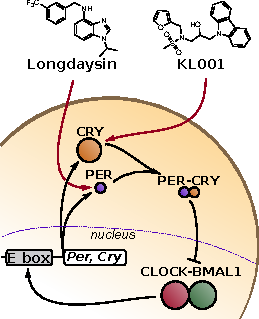
\includegraphics[width=0.4\textwidth]{chap4/figures/fig1_schem.pdf}
  \titlecaption{Small molecule targets}{Schematic of the core circadian feedback loop, with the targets of small molecule modulators longdaysin (CKI inhibitor) and KL001 (inhibitor of FBXL3-dependent CRY degradation) shown. The size of each molecule is representative of relative concentration. Figure reprinted from \cite{St.John2014}.}
  \label{fig:4-1a}
\end{figure}

\section{Results}

\subsection{Opposite amplitude effects of longdaysin and KL001}
To gain a more detailed understanding of the roles of CKI-PER and FBXL3-CRY pathways, we applied small molecule compounds longdaysin and KL001, which cause stabilization of PER and CRY, respectively \cite{Hirota2010, Hirota2012} (\fref{fig:4-1a}). 
We used {\it Bmal1}- and {\it Per2-dLuc} as circadian reporters, which represent different loops of the core clock mechanism and show circadian luminescence rhythms with mutually opposite phase. 
Time-course data on circadian reporter expression under increasing concentrations of longdaysin and KL001 \cite{Hirota2012} was analyzed for period and amplitude change (\fref{fig:4-1b}).
Longdaysin caused dose-dependent increases in period and detrended amplitude to $\approx 50\%$ of control values in both {\it Bmal1}- and {\it Per2-dLuc} reporter cells. 
In contrast, KL001 induced a simultaneous increase in period and strong reduction in amplitude. 
Modulation of the activity of CKI-PER and FBXL3-CRY is therefore differentiated by an opposite amplitude response.

\begin{figure}[h]
  \centering
  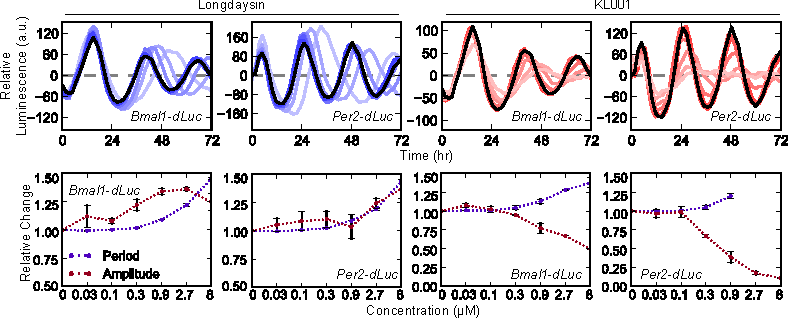
\includegraphics[width=\textwidth]{chap4/figures/fig1_ts.pdf}
  \titlecaption{Different amplitude effect of small molecule circadian modulators targeting CKI-PER and FBXL3-CRY}{(top) Detrended luminescence profiles (first 72 hours, mean of two independent replications) obtained from U2OS reporter cells with increasing concentration of longdaysin and KL001. Black profiles indicate control conditions (0 $\mu$M), lighter colors indicate higher concentrations of small molecule (from 0.03 to 8 $\mu$M). (bottom) Relative change in period and amplitude of the results in shown on top. Figure reprinted from \cite{St.John2014}.}
  \label{fig:4-1b}
\end{figure}

\subsection{Main period-determining perturbations}

We next used {\it in silico} modeling to gain mechanistic insight into CKI-PER and FBXL3-CRY mediated circadian regulation. 
In \fref{chap:model}, we describe the connection between inhibition of FBXL3-dependent CRY degradation and period change \cite{Hirota2012}: increasing the stability of nuclear CRY results in longer transcriptional repression and increased period length. 
However, while CKI has been linked to modulating PER stability and nuclear entry, it remained unclear which perturbation dominates the period effect, and whether these processes are sufficient to separate the effects of CKI and FBXL3.

To generate predictions that are consistent across slight differences in model assumptions, we chose three mathematical models from the literature based on their moderate size and similar scope \cite{Hirota2012, Leloup2003, Relogio2011}. 
The models included, at a minimum, the expression and nuclear entry mechanisms of PER and CRY. 
We considered the formation of the PER-CRY heterodimer as a key step in nuclear entry, which is supported by the fact that, to the best of our knowledge, all circadian models that consider both PER and CRY employ this kinetic assumption \cite{Hirota2012, Relogio2011, Leloup2003, Forger2003, Mirsky2009}.

Since dynamic models of genetic regulatory networks typically suffer from poor parameter identifiability \cite{Gunawan2006}, we demonstrate that our predictions are parameter-independent by employing a bootstrap identifiability analysis \cite{St.John2013}. 
As part of the bootstrap method, the models were re-fit to experimental data \cite{Lee2001} while ensuring appropriate protein stoichiometry. 
The state trajectories of the resulting 2000 parameter sets for each model are shown in \fref{fig:4.2}, with reasonable agreement between models and experiment.

\begin{figure}[h]
  \centering
  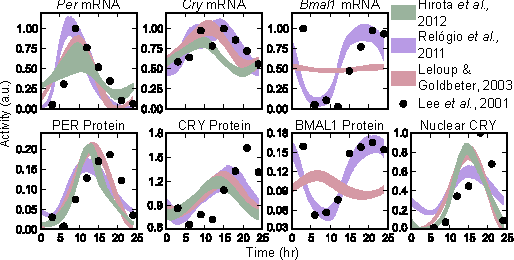
\includegraphics[width=0.8\textwidth]{chap4/figures/fig2.pdf}
  \titlecaption{Fitted trajectories from bootstrap runs}{Time series trajectories of the 2000 bootstrap trials for each model. Shaded regions indicate 95\% confidence regions. The data were scaled to have a maximum value of 1, except for protein species, where relative values were important for clock stoichiometry. Figure reprinted from \cite{St.John2014}.}
  \label{fig:4.2}
\end{figure}


A first-order period sensitivity analysis, performed on each of the parameter sets, identified which parameters associated with PER and CRY protein activity had the greatest effect on period (\fref{fig:4.s2}). 
To simplify analysis, we present only those parameters that are associated with experimentally supported mechanisms of CKI and FBXL3 in \fref{fig:4.3}. 
We first tested parameters associated with potential FBXL3-CRY activity to evaluate if our method matched the experimentally verified effect of KL001 \cite{Hirota2012}. 
Since CRY is the dominant repressor of CLOCK-BMAL1 \cite{Ye2011}, we attribute degradation rates of the PER-CRY complex to be representative of CRY clearance rates. 
We found that only parameters governing nuclear CRY degradation show a period lengthening effect upon inhibition, while rates associated with cytoplasmic CRY degradation show period shortening effects. 
These results match with our previous assertion that period lengthening occurs via nuclear CRY stabilization \cite{Hirota2012}. 
Experimental evidence has also indicated cytoplasmic CRY stabilization may lead to period shortening \cite{Kurabayashi2010}, a result consistent with our mathematical results.

\begin{figure}[p]
  \centering
  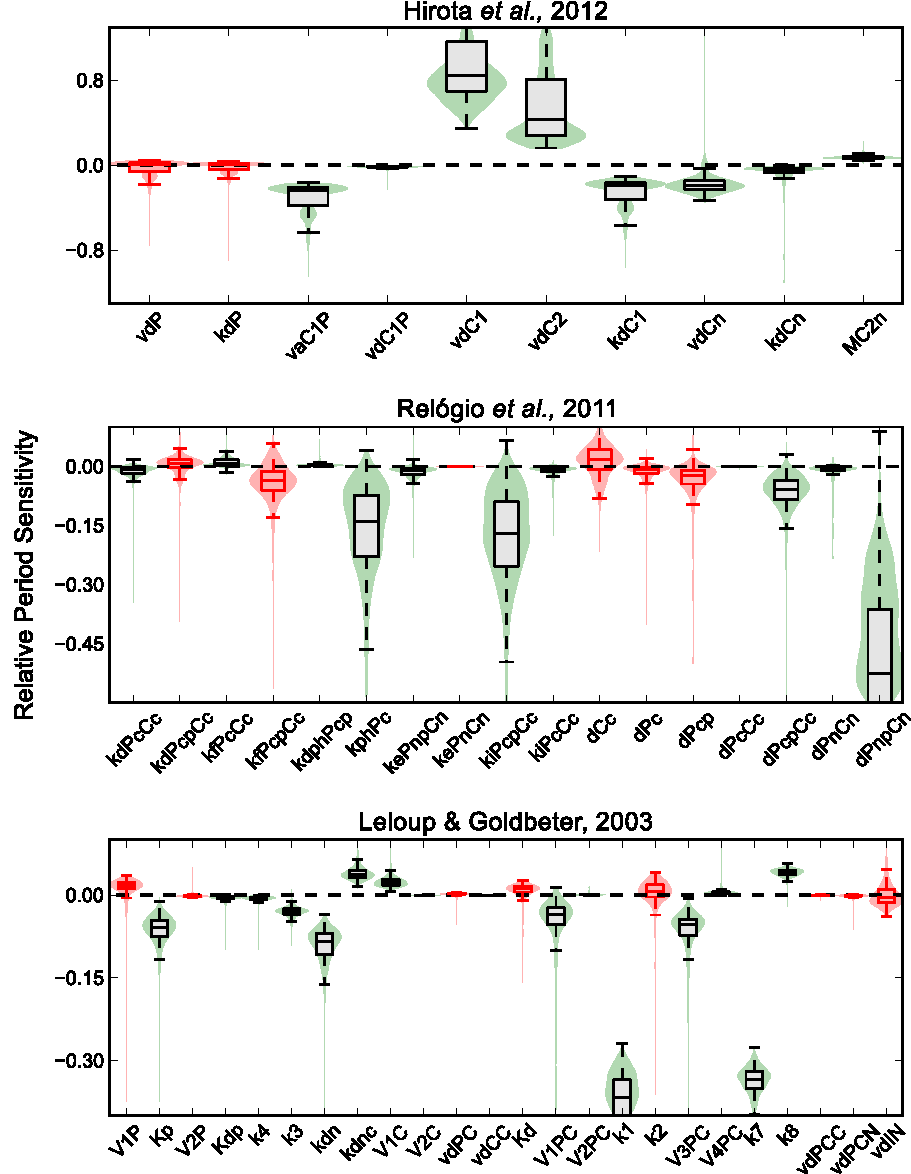
\includegraphics[height=0.7\textheight]{chap4/figures/figS2.pdf}
  \titlecaption{Bootstrap confidence intervals in relative period sensitivities}{Violin plots for distributions in relative period sensitivities for parameters associated with PER and CRY proteins. Whiskers extend to the most extreme data point within 1.5$x$ the inner quartile range.  Distributions in which the 5\textsuperscript{th} and 95\textsuperscript{th} percentile lie on opposite sides of the $x$-axis are colored red and deemed non-identifiable. Figure reprinted from \cite{St.John2014}.}
  \label{fig:4.s2}
\end{figure}

\begin{figure}[p]
  \centering
  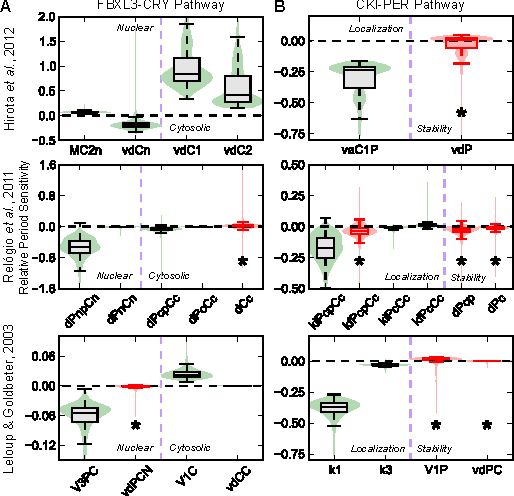
\includegraphics[height=0.6\textheight]{chap4/figures/fig3.pdf}
  \titlecaption{Bootstrap predictions of circadian actions of FBXL3-CRY and CKI-PER pathways}{Violin plots of the relative period sensitivity of parameters associated with potential mechanisms for FBXL3-CRY (A) and CKI-PER (B) activity. A negative or positive period sensitivity indicate that the period of oscillation will increase or decrease when that rate is inhibited, respectively. Distributions that are not different than 0 with 95\% confidence are colored red.  Descriptions of the parameters shown are listed in tables \ref{tab:4.1}-\ref{tab:4.2}. Figure reprinted from \cite{St.John2014}.}
  \label{fig:4.3}
\end{figure}

\begin{table}[p]
\caption{Descriptions of the model parameters governing FBXL3-CRY}
\label{tab:4.1}
\centering
\begin{tabular}{llp{10cm}}\toprule
Model              & Parameter & Description \\\midrule
\cite{Hirota2012}  & MC2n      & CRY2 nuclear multiplicative degradation coefficient \\
                   & vdCn      & CRY1/2 nuclear degradation rate \\
                   & vdC1      & CRY1 cytoplasmic degradation rate \\
                   & vdC2      & CRY2 cytoplasmic degradation rate \\\midrule
\cite{Relogio2011} & dPnpCn    & Phosphorylated PER-CRY complex nuclear degradation rate \\
                   & dPnCn     & PER-CRY complex nuclear degradation rate \\
                   & dPcpCc    & Phosphorylated PER-CRY complex cytoplasmic degradation rate \\
                   & dPcCc     & PER-CRY complex cytoplasmic degradation rate \\
                   & dCc       & CRY cytoplasmic degradation rate \\\midrule
\cite{Leloup2003}  & V3PC      & PER-CRY complex nuclear phosphorylation rate \\
                   & vdPCN     & Phosphorylated PER-CRY complex nuclear degradation rate \\
                   & V1C       & CRY cytoplasmic degradation rate \\
                   & vdCC      & Phosphorylated CRY cytoplasmic degradation rate \\\bottomrule
\end{tabular}
\end{table}

\begin{table}[p]
\caption{Descriptions of the model parameters governing CKI-PER}
\label{tab:4.2}
\centering
\begin{tabular}{llp{10cm}}\toprule
Model              & Parameter & Description \\\midrule
\cite{Hirota2012}  & vaC1P   & PER-CRY complex nuclear entry rate \\
                   & vdP     & PER cytoplasmic degradation rate \\\midrule
\cite{Relogio2011} & kiPcpCc & Phosphorylated PER-CRY complex nuclear entry rate \\
                   & kfPcpCc & Phosphorylated PER-CRY complex association rate \\
                   & kiPcCc  & PER-CRY complex nuclear entry rate \\
                   & kfPcCc  & PER-CRY complex association rate \\
                   & dPcp    & Phosphorylated PER cytoplasmic degradation rate \\
                   & dPc     & PER cytoplasmic degradation rate \\\midrule
\cite{Leloup2003}  & k1      & PER-CRY complex nuclear entry rate \\
                   & k3      & PER-CRY complex association rate \\
                   & V1P     & PER cytoplasmic phosphorylation rate \\
                   & vdPC    & Phosphorylated PER cytoplasmic degradation rate \\\bottomrule
\end{tabular}
\end{table}

We next describe parameters potentially associated with CKI-dependent regulation of PER localization and stability. 
Since PER is rate-limiting in the formation of the PER-CRY complex \cite{Lee2001}, rates associated with complex formation or nuclear import were included in this analysis. 
Conversely, we did not include degradation rates of PER-CRY nuclear repressive complex, since CRY alone is considered the main repressor. 
While it was hypothesized in models where PER acts as a direct repressor that the regulation of PER stability would play the dominant role determining the period \cite{Gallego2006, Vanselow2006}, our new assumptions revealed that parameters governing PER degradation showed only non-identifiable responses. 
 However, inhibition of rates associated with the nuclear entry of the PER-CRY complex showed strong period lengthening effects. 
These results indicate that under our current understanding of clock kinetics, the regulation of nuclear import likely plays the prominent role in CKI-dependent period regulation.

\subsection{Independent mechanisms of PER and CRY regulation}
Using \fref{mod:hirota} and the perturbations identified in \fref{fig:4.3}, we first confirmed that inhibition of nuclear CRY degradation (vdCn) and PER-CRY nuclear import (vaC1P) reproduced the experimental period and amplitude effects of the small molecules KL001 and longdaysin, respectively (\fref{fig:44a}, compare with \fref{fig:4-1b}). 

\begin{figure}[h]
  \centering
  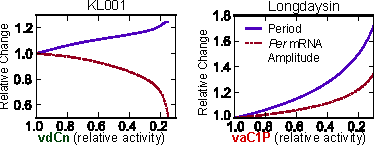
\includegraphics[width=0.7\textwidth]{chap4/figures/fig4a.pdf}
  \titlecaption{Predictions of KL001 and longdaysin results}{{\it In silico} reproductions of the circadian reporter experiments in \fref{fig:4-1b}, using the predictions identified in \fref{fig:4.3}. Figure reprinted from \cite{St.John2014}.}
  \label{fig:44a}
\end{figure}

Comparison of the oscillatory profiles of {\it Per} mRNA and nuclear CRY protein (\fref{fig:44b}) revealed that inhibition of FBXL3-dependent CRY degradation caused lingering nuclear CRY to not be completely purged each cycle. 
 This excess repressor during the accumulating phase of {\it Per} and {\it Cry} transcripts resulted in lower E box amplitudes, providing a likely explanation for the effect of KL001.

\begin{figure}[h]
  \centering
  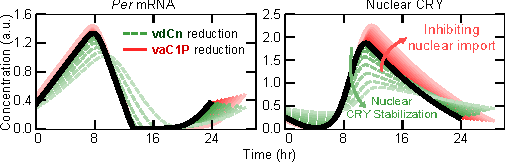
\includegraphics[width=0.85\textwidth]{chap4/figures/fig4b.pdf}
  \titlecaption{Comparison of the effects of KL001 and longdaysin}{Parameter changes were normalized such that the period change was equal for each pair of perturbations (vdCn: 100\% $\to$ 23\%, vaC1P: 100\% $\to$ 51\%). Figure reprinted from \cite{St.John2014}.}
  \label{fig:44b}
\end{figure}

In contrast, stabilization of cytoplasmic PER (lowering vdP) resulted in reduced transcriptional amplitude with minimal period effect (\fref{fig:4S3}), consistent with experimental findings from the knockdown of $\beta$-TrCP, an F box protein responsible for PER degradation \cite{Ohsaki2008}. 
However, other experimental results have shown that down-regulation of $\beta$-TrCP leads to longer periods \cite{Reischl2007}, suggesting that further modeling and experimental inquiry is needed on the role of $\beta$-TrCP in clock regulation. 
This period lengthening might be explained through $\beta$-TrCP-mediated stabilization of nuclear PER-CRY or by using alternative kinetic assumptions for the rate of PER-CRY binding. 

\begin{figure}[h]
  \centering
  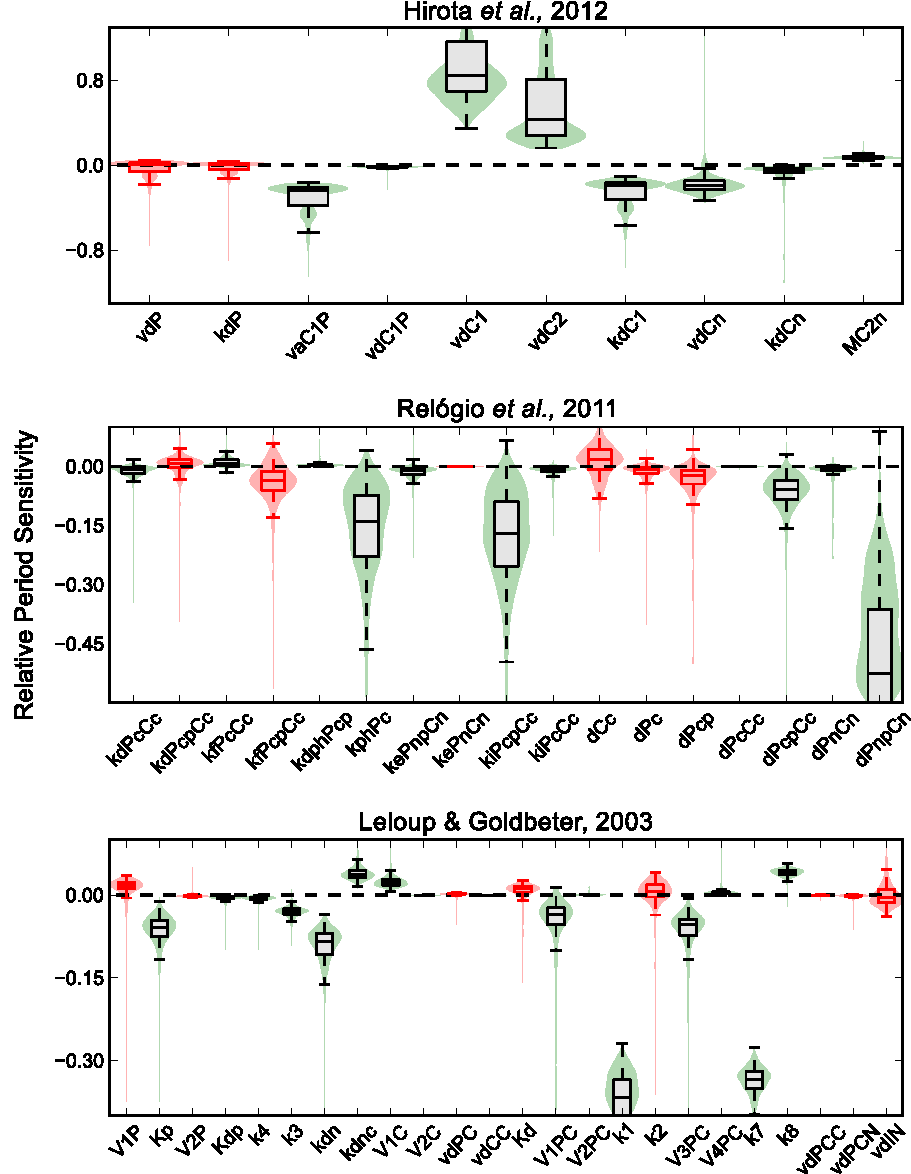
\includegraphics[width=0.6\textwidth]{chap4/figures/figS3.pdf}
  \titlecaption{Effect of cytoplasmic PER stabilization on period and E box transcription amplitude}{Relative period and peak-to-trough amplitude change in {\itshape Per} mRNA resulting from a reduction in the vdP parameter in the model from Hirota {\itshape et al.}, 2012. Figure reprinted from \cite{St.John2014}.}
  \label{fig:4S3}
\end{figure}


\subsubsection{CKI likely regulates nuclear entry rather than PER stability}
We further compared the effect of inhibiting PER degradation with inhibiting nuclear import on the oscillatory profile of key clock proteins (\fref{fig:44c}) to identify mechanistic differences between the two potential effects of CKI inhibition. 
Both perturbations increased cytoplasmic PER, suggesting the two mechanisms are difficult to distinguish experimentally. 
Direct stabilization of PER in the cytoplasm (lowering vdP) lead to two simultaneous trends which shift the period in opposite directions: it shortened the time delay between transcription and inactivation by accelerating the accumulation of cytoplasmic PER and nuclear PER-CRY; and lengthened the repressive phase by increasing the total amount of PER-CRY which enters the nucleus. 
These perturbations sped and slowed the clock, respectively, and resulted in little period change. 
In contrast, inhibiting PER-CRY nuclear entry (lowering vaC1P) caused additional free protein to build in the cytoplasm, delaying nuclear accumulation and ultimately increasing the total amount of nuclear PER-CRY. 
Since both of these trends work to increase period length, inhibiting PER-CRY nuclear entry resulted in significantly longer cycles. 
Additionally, the longer cytoplasmic time delay resulted in increased transcription, yielding slightly higher amplitudes (\fref{fig:44b}) that closely match the experimental results of the small molecule longdaysin.

\begin{figure}[h]
  \centering
  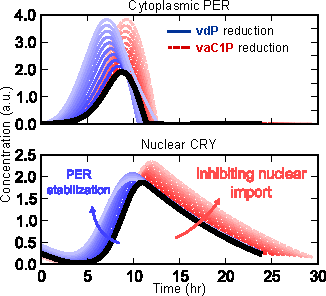
\includegraphics[width=0.6\textwidth]{chap4/figures/fig4c.pdf}
  \titlecaption{Comparison of two candidate mechanisms for CKI inhibition}{Effects of increasing PER stabilization and nuclear import inhibition  on the time profiles of cytoplasmic PER (top) and nuclear CRY (bottom). Parameter values were selected such that the amplitudes of cytoplasmic PER are equal at each level. Lighter colors indicate stronger perturbations (vdP: 100\% $\to$ 22\%, vaC1P: 100\% $\to$ 45\%), $t=0$ is set to the onset of PER accumulation. Figure reprinted from \cite{St.John2014}.}
  \label{fig:44c}
\end{figure}


Since CKI likely regulates both stability and subcellular localization of PER {\it in vivo}, we considered the effects of simultaneously lowering both PER cytoplasmic degradation and nuclear entry rates, as shown in \fref{fig:45}.
The loss of oscillations under extreme reduction of both parameters highlights an interesting role of CKI in conferring robustness to the circadian clock: since oscillations are lost when import of the PER-CRY complex to the nucleus ceases to be rhythmic, CKI ensures lingering PER is purged from the cytoplasm by one pathway or another before E box transcription resumes. 
This importance has been proven experimentally, as disruption of CKI-mediated regulation leads to compromised circadian oscillations \cite{Lee2009a}.


\begin{figure}[h]
  \centering
  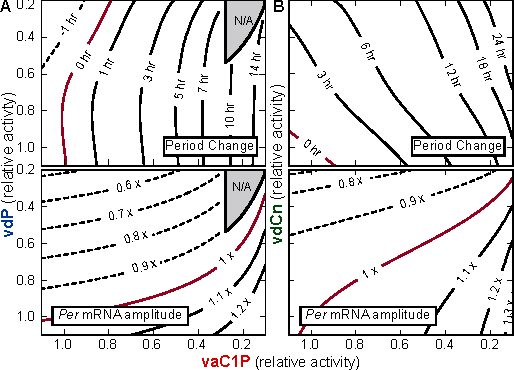
\includegraphics[width=0.9\textwidth]{chap4/figures/fig5.pdf}
  \titlecaption{Independence of CKI-PER and FBXL3-CRY pathways}{({\bfseries A}) Contour plots of period change (top) and {\bfseries Per} mRNA amplitude (bottom) for simultaneous inhibition of both PER degradation (vdP) and nuclear import (vaC1P). The gray shaded region indicates loss of oscillations. ({\bfseries B}) Period and amplitude change contour plots for varying both vdCn (CRY nuclear degradation rate) and vaC1P (PER-CRY nuclear import). The consistently straight lines indicate the independence of CKI-PER and FBXL3-CRY mechanisms. Figure reprinted from \cite{St.John2014}.}
  \label{fig:45}
\end{figure}

Together, inhibition of CKI by longdaysin may increase the time required before PER-CRY can enter the nucleus to repress transcription, leading to a higher amplitude and longer period. 
In contrast, KL001 lengthens the period by stabilizing nuclear CRY, resulting in a longer time delay before transcription resumes and lower amplitude from increased E box repression. 
PER regulation through CKI is therefore partitioned to the accumulating phase, controlling the speed and amount of PER-CRY complex that enters the nucleus. 
CRY regulation through FBXL3 is partitioned independently to the repressive phase, controlling the length of time until CLOCK-BMAL1-dependent transcription resumes (\fref{fig:46}). 
This independence was reproduced {\it in silico} by the simultaneous reduction of nuclear CRY degradation and PER-CRY nuclear import (\fref{fig:45}), where nonlinear interactions in amplitude and period between the two perturbations are all but absent.

\begin{figure}[h]
  \centering
  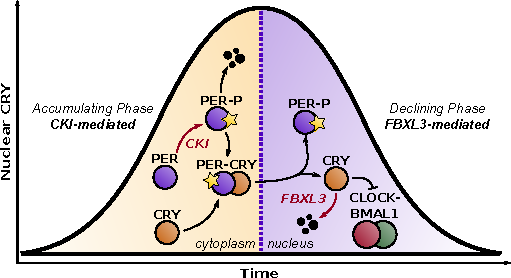
\includegraphics[width=0.8\textwidth]{chap4/figures/fig6.pdf}
  \titlecaption{Spatiotemporal separation underlies independence of CKI-PER and FBXL3-CRY pathways}{Longdaysin, acting through CKI, lengthens the accumulating phase of the circadian cycle, while KL001, acting through FBXL3, lengthens the declining phase. Figure reprinted from \cite{St.John2014}.}
  \label{fig:46}
\end{figure}

\section{Discussion}
An understanding of the interactions between posttranslational regulators is crucial for the further development of circadian pharmacological reagents, as efficient modulation of clock function will assuredly come from simultaneous perturbations to many connected species. 
In this study, we used circadian reporter cells together with mathematical modeling to provide mechanistic insight into the differences of CKI- and FBXL3- mediated posttranslational regulation of PER and CRY. 
As a result, we clarified a process by which CKI exerts control over the circadian period, demonstrated through both the hyperphosphorylating CKI$\epsilon^\mathrm{tau}$ mutant and small molecule CKI inhibitors, such as longdaysin. 
In developing our predictions, we have used multiple models and parameterizations to ensure our mechanisms are consistent across many {\it in silico} realizations. 
These results reinforce the notion that computational modeling is essential in interpreting results in systems with complicated oscillatory feedback. 
Additionally, {\it in silico} analyses reveal hidden design principles of biological networks, as this work highlights the importance of the CKI family of kinases in conferring robustness to the circadian cycle. 
 
\subsection{Phase-dependent activity of small molecule modulators}
In this chapter, it was shown that the posttranslational CKI and FBXL3 control separate time regimes of the core clock oscillation. 
While in the cultured cell experiments the small molecule modulators were continuously present, in pharmacological applications there would likely be dosed at specific times of day. 
Since their targets play key roles during specific circadian phases, it is likely that there would be a significant difference in small molecule effect depending on the time at which they are given. 
In the next chapter, we systematically analyze the dynamic consequences associated with {\itshape transient} applications of small molecule agonises, rather than dose-dependent continuous applications, as the former will likely have more significant clinical relevance. 
